\chapter{A análise dos dados}\label{chp:CAP_ANALISE}

O escopo inicial deste trabalho propôs 4 diferentes análises:

\begin{enumerate}

\item \textbf{Frequência da linha}: calcula qual foi a frequência e tempo médio de espera por ônibus de uma linha. Reflete quanto tempo um usuário costuma esperar, em média, até que passe seu ônibus, em cada horário do dia. Pode ser usada para comparação com a frequência informada por cada companhia e para o próprio usuário poder estimar o tempo que irá aguardar até embarcar.

\item \textbf{Concentração da frota}: mostra onde os ônibus estiveram nas últimas 24 horas, mostrando quais regiões possuem maior concentração de ônibus e quais sequer possuem linhas de ônibus.

\item \textbf{Quantidade de ônibus por linha e hora}: similar ao estudo anterior, porém  mostra quantos carros de cada linha estavam circulando em cada horário do dia. Pode ser comparada com a quantidade de veículos determinada nas concessões da Prefeitura às companhias de ônibus.

\item \textbf{Atualização do GPS}: uma meta-análise dos DAGs para monitorar a qualidade do monitoramento dos ônibus em relação à atualização dos dados. Pode servir pra mostrar quais companhias não estão transmitindo os dados de sua frota e, portanto, descumprindo seu contrato com a Prefeitura.

\end{enumerate}

Foram desenvolvidos os estudos 1 e 2, que serão descritos em detalhes a seguir.


\renewcommand{\labelenumii}{\theenumii}
\renewcommand{\theenumii}{\theenumi.\arabic{enumii}.}

\section{Frequência dos ônibus}

Este estudo tem como objetivo analisar a frequência dos ônibus de uma linha, de maneira que o resultado final reflita qual o tempo médio de espera por um ônibus daquela linha em um certo horário do dia. Tal informação não é oferecida pelos DAGs utilizados e, apesar de algumas companhias de ônibus divulgarem uma frequência oficial de suas linhas, muitas vezes estas não são cumpridas ou, na prática, são afetadas por outros fatores, como o trânsito.


\subsection{Dados utilizados}

As estatísticas são obtidas a partir de uma amostra dos registros de localização dos ônibus em um período de 24 horas. Como as linhas possuem diferentes características, cada linha foi analisada individualmente e os dados médios serão agrupados por hora.

Também são usados para compreensão desses dados a informação geolocalizada dos pontos de parada da linha.


\subsection{O algoritmo}

Calcularemos o intervalo de tempo entre cada ônibus da linha em diversos pontos ao longo do itinerário. Considere disponíveis as variáveis e funções abaixo:

\begin{itemize}
    \item $L$: a linha a ser analisada (ex.: $485$);
    \item $D$: a data a ser analisada (ex: $08/10/2015$);
    \item $stops(L)$: função que retorna o conjunto de pontos de parada geolocalizados da linha $L$;
    \item $history(L,D)$ a função que retorna os registros geolocalizados dos ônibus da linha $L$ na data $D$;
    \item $matches(R,p)$ a função que retorna o subconjunto dos registros $R$ próximos a um ponto de parada $p$.
\end{itemize}

O algoritmo desenvolvido é descrito a seguir.

\begin{enumerate}

\item Obter $P = stops(L)$ e $R = history(L,D)$.
%\item Obter as informações dos pontos de parada da linha e as posições dos ônibus da linha selecionada, para o dia analisado.

\item Para cada ponto $p_i$ de $P$: 

    \begin{enumerate}
        \item Obter $M_i = matches(R,p_i)$, isto é, os registros dos ônibus que passaram pelo ponto de parada $p_i$.
        
        \item Ordenar $M_i$ pelo horário dos registros de forma ascendente.\footnote{Obtém-se ao final da ordenação a sequência de cada ônibus que passou por aquele ponto ao longo do dia - assim como teria, por exemplo, um fiscal da companhia de ônibus, cuja função é anotar os horários em que cada ônibus da companhia passou por ali.}
        
        \item Eliminar de $M_i$ registros de um mesmo ônibus com horários próximos, a fim de evitar que ele seja contado mais de uma vez.\footnote{Caso o ônibus encontre-se parado durante muito tempo no ponto ou próximo a ele, pode haver mais de um registro, cujos cruzamentos duplicados devem ser descartados.}
        
        \item Dividir os cruzamentos de $M_i$ em 24 subconjuntos $M_{ij}$ de acordo com a hora de cada registro ao longo do dia.
        
        \item Para cada conjunto $M_{ij}$, $0 \leq j < 24$, calcular o intervalo de tempo entre cada registro do conjunto e a média $I_{ij}$ dos intervalos.
        
    \end{enumerate}
    
\item Para cada hora do dia, $0 \leq j < 24$, calcular a média entre todos os pontos $i$ dos intervalos $I_{ij}$. 

\end{enumerate}

Ao fim do algoritmo, obtém-se um conjunto com 24 médias, representando o intervalo médio - ou seja, a frequência - dos ônibus daquela linha em cada hora do dia.

O motivo de a frequência dos ônibus ser analisada por hora é devido ao próprio modelo de funcionamento das linhas, que possui frequências variáveis de acordo com a demanda de cada horário.

Através do algoritmo mostrado, também é possível calcular qual foi o tempo de retorno do ônibus, indicando o tempo total de viagem na linha (ida + volta). Para isso, basta calcular o tempo entre duas ocorrências do mesmo ônibus no mesmo ponto e com o mesmo sentido - ou seja, o tempo que o ônibus levou desde que passou ali até percorrer a linha toda e passar ali de novo.


\subsection{Implementação}

O algoritmo foi implementado em Node.js, que é um ambiente de desenvolvimento em JavaScript\cite{REF_JAVASCRIPT}\cite{REF_NODEJS}. Essa escolha foi feita principalmente devido à velocidade do desenvolvimento e por ser uma boa linguagem de prototipagem\cite{REF_NODEJS_PROTOTYPING} e possui um excelente suporte ao MongoDB, banco de dados utilizado.

Foi desenvolvido um programa que faz a conexão com o banco de dados, já populado, executando o algoritmo acima e exportando os dados calculados para um arquivo JSON. 

Também foi criada uma página HTML\cite{REF_HTML} que usa JavaScript para ler os dados do arquivo JSON e plotá-los num gráfico de barras, a fim de facilitar a visualização dos dados de hora em hora ao longo do dia analisado.


\subsection{Resultados observados}

Foi utilizado como exemplo do estudo o histórico de julho de 2015 da linha 324, que faz o percurso Ribeira (Ilha do Governador) x Candelária (Centro). Segundo o site da empresa que controla essa linha, a Viação Ideal, a frequência média oficial é de 9 minutos entre cada ônibus\cite{ideal_324}.

Na figura \ref{fig:LABEL_FIG_ANALISE_FREQ_324}, os dados analisados são de um dia útil. Podemos observar durante a manhã desse dia que o tempo médio de espera por um ônibus dessa linha fica em torno de 20 minutos, com pequenos aumentos chegando a 25 minutos para quem aguardava um ônibus entre as 8 e 10 horas, período com reflexos do horário do rush. Já na faixa das 12 horas, nenhuma média foi calculada, pois não houve frequência suficiente de ônibus nos pontos analisados para que o algoritmo pudesse calcular uma média. Durante o começo da tarde, vemos um grande aumento no tempo de espera, provavelmente causado pelo mesmo motivo que causou a falta de dados no período das 12 horas, que foi normalizando nas horas seguintes até que aumentou de novo a partir das 19 horas.

Uma comparação da análise desse dia pode ser feita com a da figura \ref{fig:LABEL_FIG_ANALISE_FREQ_324_DOMINGO}, com os dados da mesma linha porém em um domingo. Duas observações podem ser feitas imediatamente: a média de espera é maior, pois aos finais de semana há menos ônibus circulando e também o tempo de espera é bem mais constante, visto que num domingo não há trânsito causando atrasos na circulação dos ônibus.

Com uma base de dados maior, é possível fazer tais comparações entre datas mais relevantes, a fim de observar os reflexos na frequência dos ônibus causados por eventos, interdições, desvios e outros fatores. Também é possível agregar dados analisados em intervalos maiores.

\begin{figure}
  \centering
  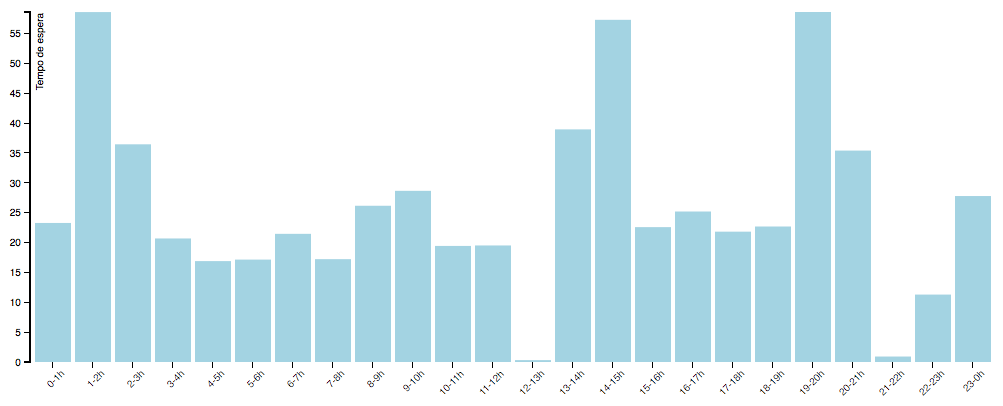
\includegraphics[width=1.0\textwidth]{imagens/grafico_freq.png}
  \caption{Análise mostra o tempo médio de espera por um ônibus da linha 324 num dia útil em julho de 2015.}
  \label{fig:LABEL_FIG_ANALISE_FREQ_324}
\end{figure}

\begin{figure}
  \centering
  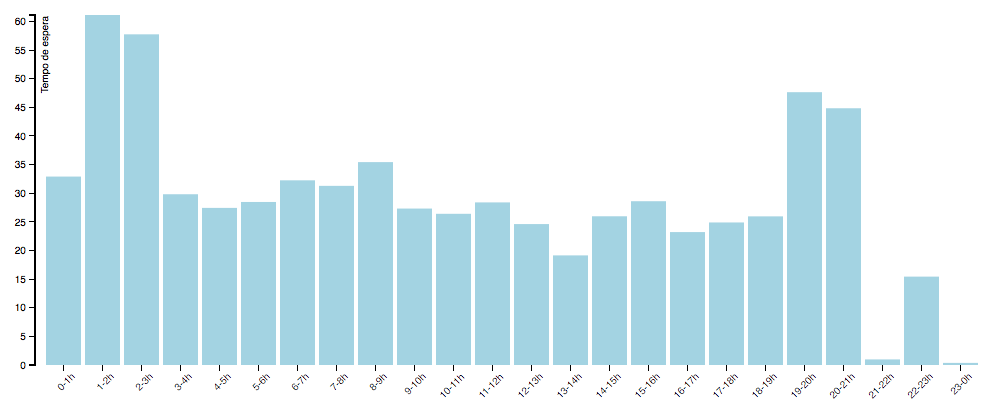
\includegraphics[width=1.0\textwidth]{imagens/grafico_freq_dom.png}
  \caption{Análise mostra o tempo médio de espera por um ônibus da linha 324 num domingo em julho de 2015.}
  \label{fig:LABEL_FIG_ANALISE_FREQ_324_DOMINGO}
\end{figure}

Apesar de o algoritmo ser relativamente simples, houve uma grande dificuldade na filtragem dos registros duplicados. Ao observar que os resultados da execução com uma certa linha estavam apontando um resultado surpreendentemente bom, notamos que existe um cenário específico em que os ônibus são erroneamente identificados cruzando um ponto de parada.

Foi comparada a execução do algoritmo em diferentes linhas com resultados similares. Concluiu-se que estava sendo computado um falso positivo dos ônibus que cruzavam um ponto de parada no sentido contrário ao esperado. Logo, observou-se que isso era um cenário recorrente nas linhas em que o itinerário de ida era similar ao itinerário de volta, como quando uma linha passa na mesma rua nos dois sentidos. Nesse caso, os pontos de parada da ida são muito próximos aos pontos da volta - às vezes com pouquíssimos metros de distância, apenas em lados opostos da rua.

O algoritmo que calcula o cruzamento de um ônibus com um ponto de parada através de seu raio de proximidade acabava identificando um falso positivo nesses casos. Visando contornar esse problema, foi necessário implementar essa diferenciação do sentido por conta própria.

A fim de identificar se um ônibus está no seu itinerário de ida ou de volta, foi elaborado um algoritmo que identifica qual o sentido comparando a posição atual do ônibus com a sua posição nos últimos registros. Considerando que conhecemos o itinerário da linha, comparamos o histórico das últimas $n$ posições conhecidas do ônibus, guardadas na memória, com o itinerário dos dois sentidos, analisando se o trajeto pertence ao conjunto da ida ou da volta.

Uma vez conhecido o sentido atual, esse dado é salvo junto ao registro do ônibus para que possa ser utilizado posteriormente. Para identificar se um determinado ônibus realmente passou por um ponto de parada, verificamos se o sentido registrado naquele instante condiz com o sentido do ponto. Caso sejam diferentes, esse registro é descartado, eliminando o falso positivo.

\section{Concentração da frota}

A proposta deste estudo é evidenciar, através de um mapa de calor, onde estão concentrados os ônibus pela cidade ao longo de um dia. Pode ser usada como ferramenta para o planejamento de novas linhas e redistribuição das atuais. 

Apesar de ser difícil extrair conclusões apenas com este mapa, ele pode servir como uma ferramenta visual para observar em que vias e regiões da cidade estão concentrados os ônibus. Um exemplo é a figura \ref{fig:LABEL_FIG_ANALISE_CONCENTRACAO_CIDADE}, que traz uma visão geral da cidade do Rio de Janeiro.

\begin{figure}
  \centering
  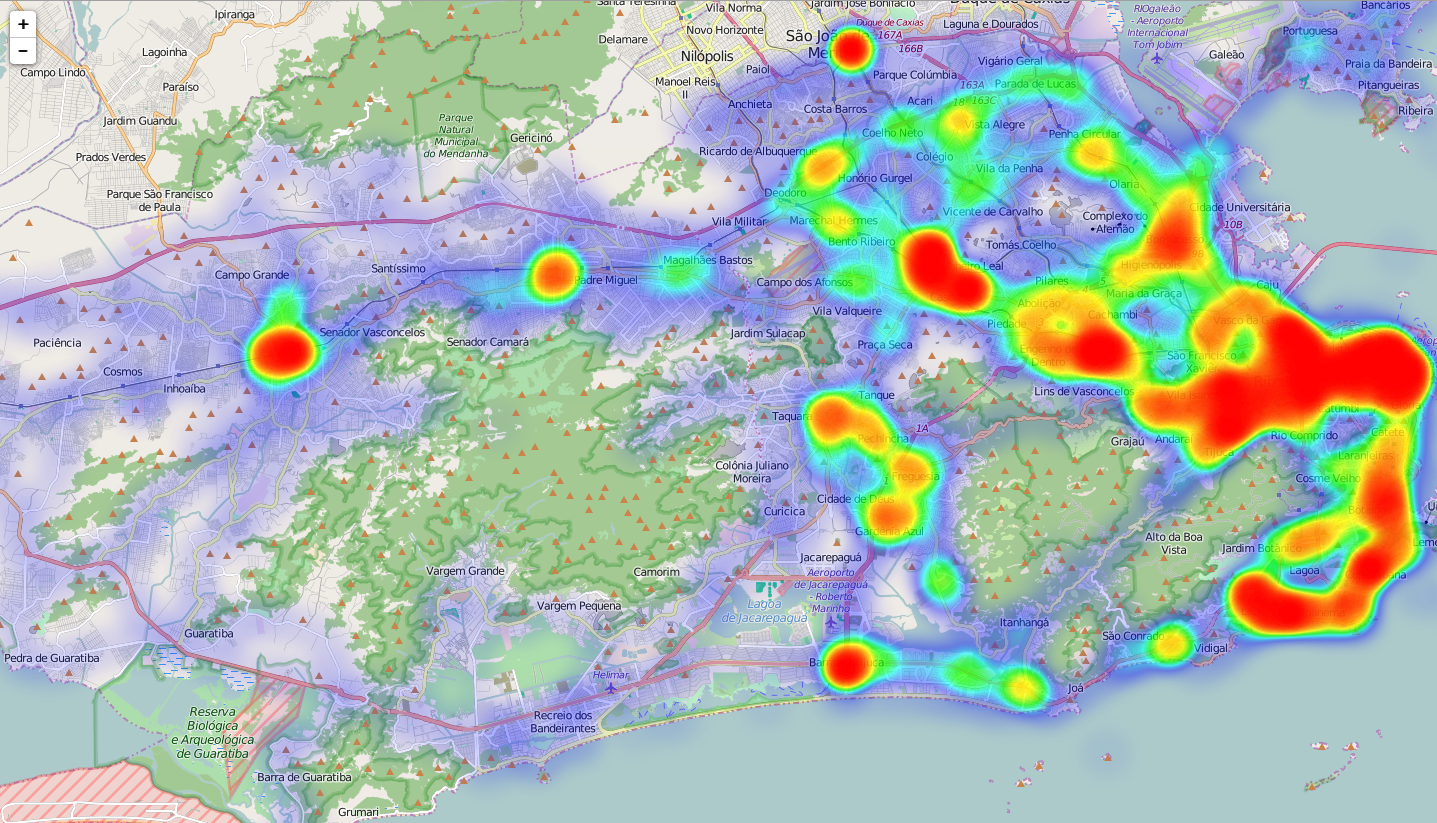
\includegraphics[width=1.0\textwidth]{imagens/heat_map1.png}
  \caption{Vista geral da cidade mostra uma grande concentração de ônibus nas regiões centrais. (Outubro de 2015)}
  \label{fig:LABEL_FIG_ANALISE_CONCENTRACAO_CIDADE}
\end{figure}


\subsection{Implementação}

Por ser uma análise mais simples, o esforço maior desta análise foi na parte da apresentação dos dados, ao invés da extração dos mesmos. 

Para extrair os dados, foi feita uma consulta no banco de dados por todos os registros geolocalizados em uma data específica. Como extrair e plotar esses dados diretamente seria muito demorado - há mais de 15 milhões de registros por dia - optamos por reduzir manualmente a precisão desses dados, agrupando registros muito próximos.

Para agrupar essas amostras, limitamos na nossa consulta a precisão dos campos de latitude e longitude de cada registro, utilizando uma precisão máxima de 4 casas decimais ao invés de 6. Só isso já reduz nosso número de amostras em cerca de 35 vezes, para cerca de 420.000 amostras, ainda mantendo uma boa precisão visual dos dados. 

Finalmente, a fim de descobrir quantos ônibus estavam em cada coordenada, foi utilizada a quantidade de registros naquela posição, contando apenas veículos distintos (cada ônibus é identificado por um número de ordem). Temos então como saída uma lista de coordenadas e suas respectivas quantidades de ônibus. 

Cada coordenada é plotada no gráfico através de uma escala de cores que representa a densidade de ônibus naquela região\cite{heatmap}. Como resultado, temos cores entre o azul escuro, que representa uma baixa densidade de ônibus na região, e o vermelho, que representa uma alta densidade. As escalas de cores foram normalizadas entre os estudos para preservar facilitar a comparação entre diferentes mapas.

Para a visualização desses dados, foi elaborada uma página que renderiza um mapa interativo, no qual é possível alterar a região de estudo e observar com maior precisão os resultados, permitindo focar em bairros ou ruas específicas. Quando duas amostras são comparadas, é possível visualizá-las lado-a-lado, atualizando simultaneamente conforme o mapa é movimentado pelo usuário.


\subsection{Resultados observados}

O mapa de calor se torna ainda mais útil quando são comparados dados de diferentes períodos, a fim de analisar como mudou a distribuição dos ônibus ao longo do tempo.

Uma das comparações feitas foi entre dados de dois anos consecutivos, 2015 e 2016. Foram analisados dados do mesmo dia, 8 de julho, um dia útil, nos dois anos. A comparação entre esses anos é especialmente relevante pois, desde o final de 2015 até a data atual, ocorrem grandes mudanças nas linhas de ônibus do Rio de Janeiro, em especial devido ao plano de racionalização das linhas da Zona Sul\cite{noticia_racionalizacao}. Além disso, devido a grandes obras pela cidade, houve diversas interdições no trajeto das linhas, a construção de novas vias e implantação de novos corredores exclusivos de ônibus.

Na figura \ref{fig:LABEL_FIG_ANALISE_RACIONALIZACAO}, é possível visualizar essa comparação e observar uma enorme diminuição dos ônibus nos bairros da Zona Sul próximos à Lagoa Rodrigo de Freitas. 

\begin{figure}
  \centering
  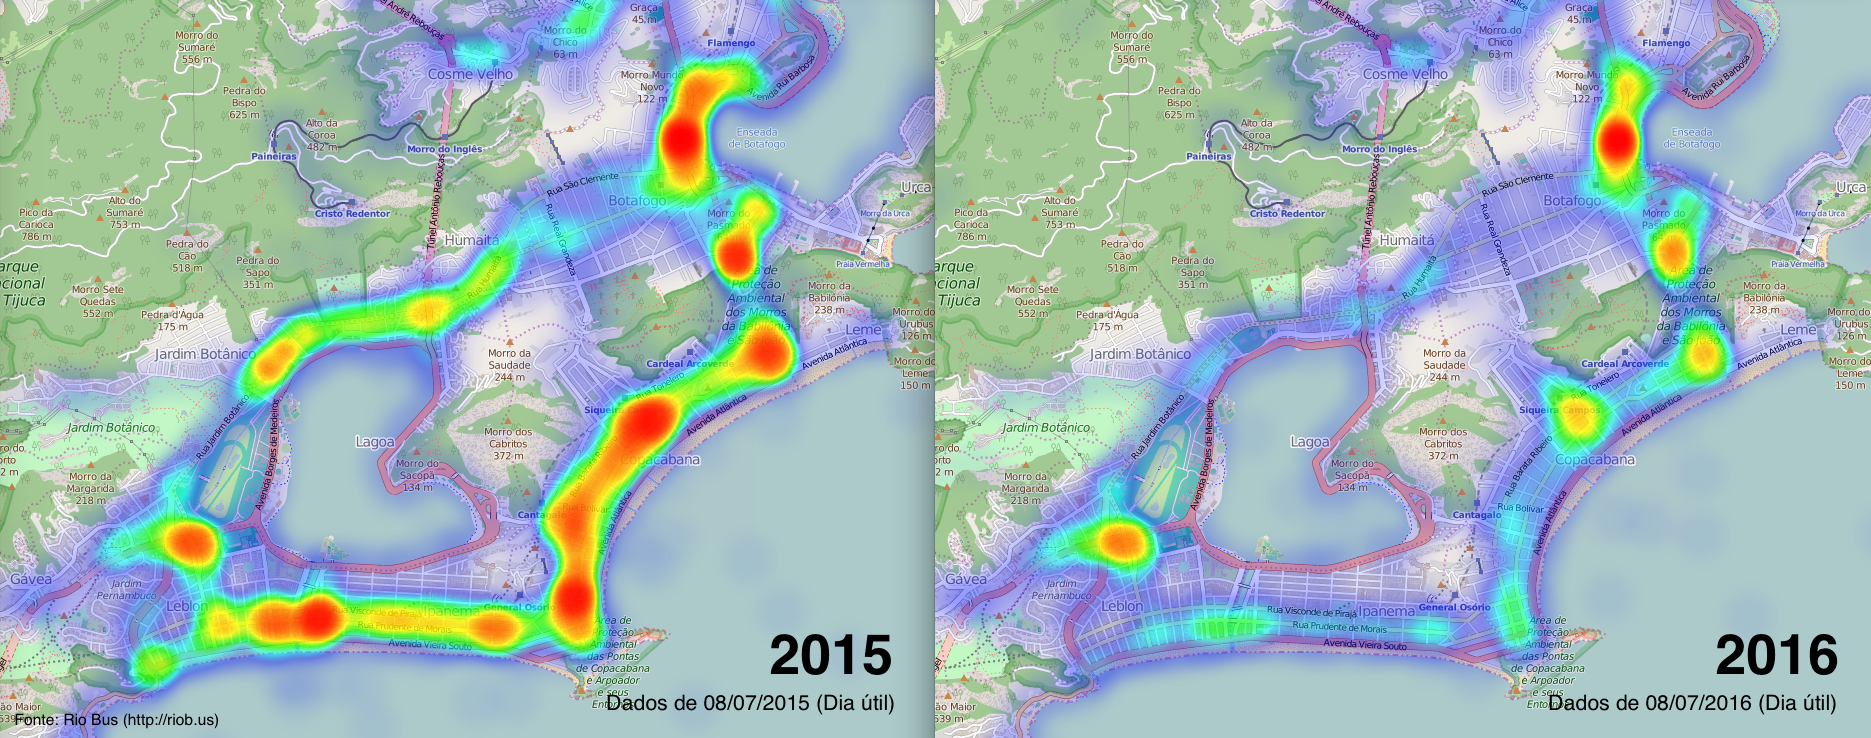
\includegraphics[width=1.0\textwidth]{imagens/heat_map_zs201516.png}
  \caption{Comparação da quantidade de ônibus na Zona Sul em dois anos consecutivos. Em 2016, observa-se a redução em virtude da racionalização das linhas de ônibus.}
  \label{fig:LABEL_FIG_ANALISE_RACIONALIZACAO}
\end{figure}


No Centro da cidade, observa-se através da figura \ref{fig:LABEL_FIG_ANALISE_CONCENTRACAO_CENTRO} que as principais vias da região concentram praticamente toda a circulação dos ônibus, enquanto vias transversais não possuem quase nenhum tráfego desse tipo.

\begin{figure}
  \centering
  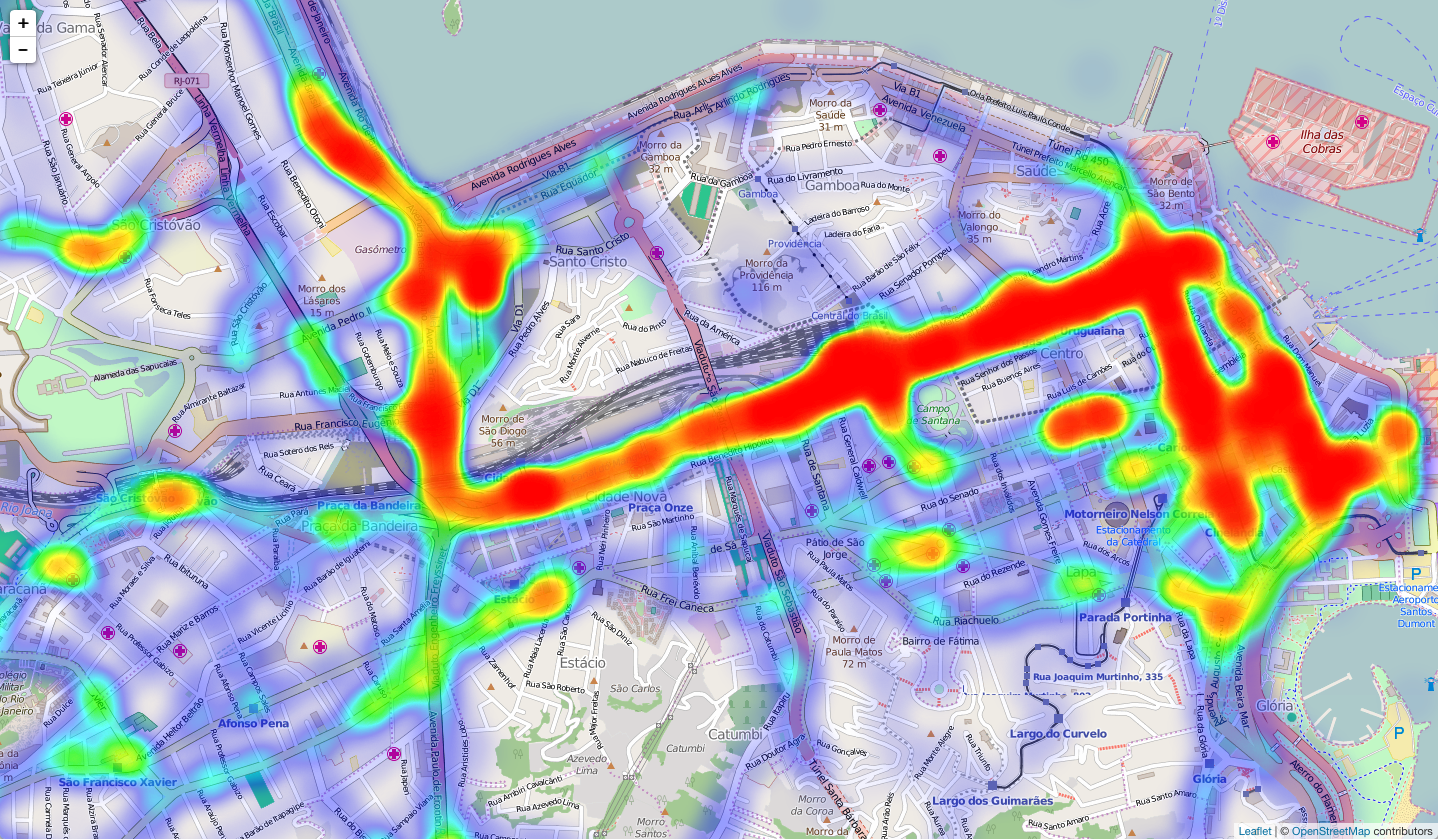
\includegraphics[width=0.9\textwidth]{imagens/heat_map2.png}
  \caption{No Centro, concentração alta nas vias principais e baixa nas transversais. (Outubro de 2015)}
  \label{fig:LABEL_FIG_ANALISE_CONCENTRACAO_CENTRO}
\end{figure}

% \begin{figure}
%   \centering
%   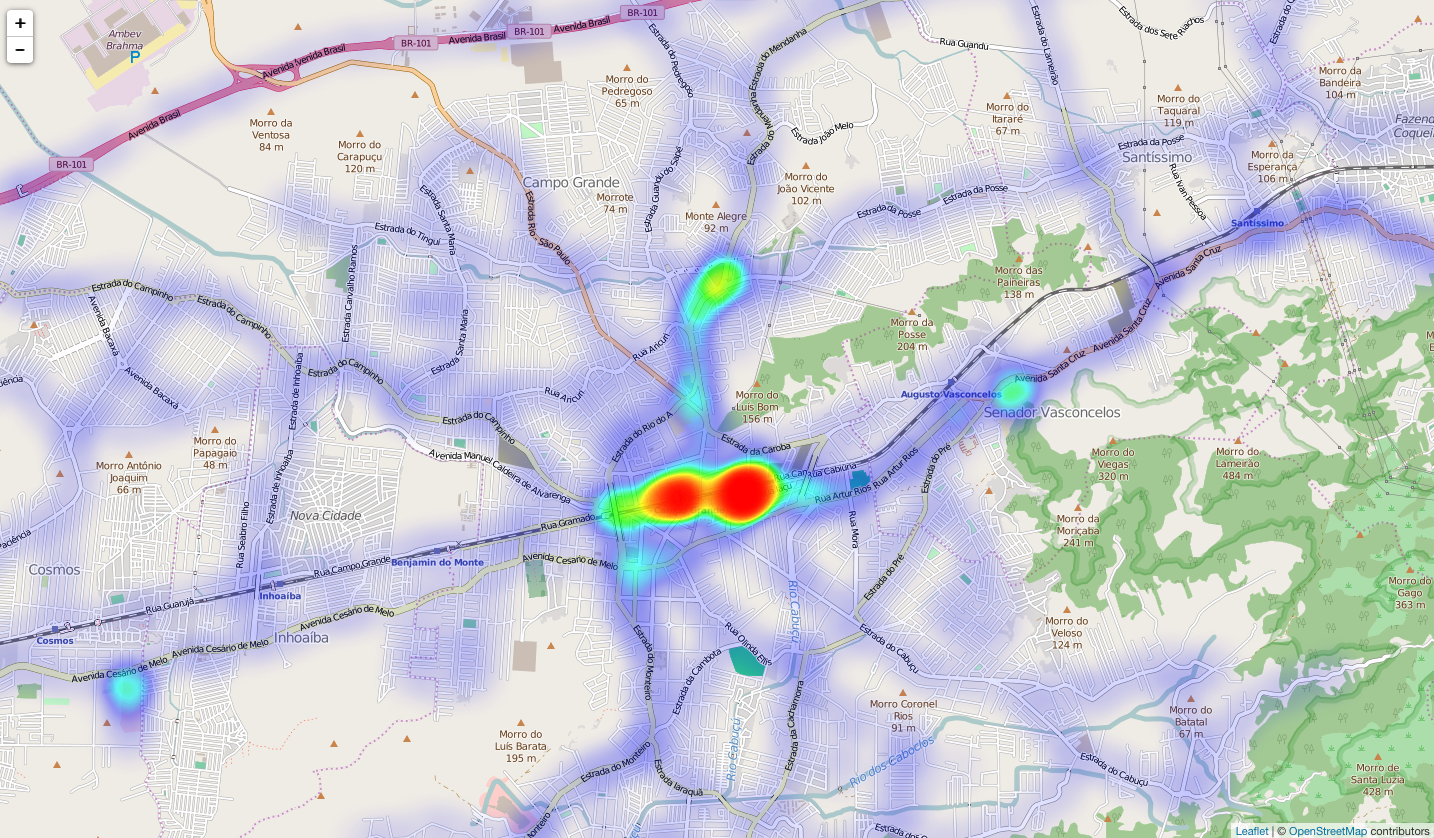
\includegraphics[width=1.0\textwidth]{imagens/heat_map3.png}
%   \caption{Enorme concentração em um único trecho em Campo Grande. (Outubro de 2015)}
%   \label{fig:LABEL_FIG_ANALISE_CONCENTRACAO_3}
% \end{figure}